%\documentclass[handout]{beamer}
\documentclass{beamer}

\usetheme{Copenhagen}

\usepackage{amsbsy}
% \usepackage{amsmath}
\usepackage{amstext}
\usepackage{amsfonts}
\usepackage{amssymb}
\usepackage{amsthm}
\usepackage{shadow}% kotak shadow
\usepackage{biblatex}

\newcommand{\R}{\mathbb{R}}
\newcommand{\E}{\mathbb{E}}
\newcommand{\RCH}{\text{RCH}}
\newcommand{\CH}{\text{CH}}
\newcommand{\Prob}{\mathbb{P}}
\newcommand{\F}{\mathcal{F}}
\newcommand{\G}{\mathcal{G}}
\newcommand{\B}{\mathcal{B}}
\newtheorem*{prop}{Proposition}
\newtheorem*{prob}{Problem}
\newcommand{\rch}{\operatorname{RCH}}

\usepackage{tikz}

\usepackage{curves}
\usepackage{graphics}
\usepackage{graphicx}
\usepackage{color}%masukan colorbegi
\usepackage{makeidx}
\makeindex

%\setbeamertemplate{footline}{}
\setbeamertemplate{footline}[frame number]
\title[Double Descent Demystified]{Double Descent Demystified: Identifying, Interpreting \& Ablating the Sources of a Deep Learning Puzzle}
\subtitle[Rylan Schaeffer, ]{Rylan Schaeffer, Mikail Khona, Zachary Robertson, Akhilan Boopathy, Kateryna Pistunova, Jason W. Rocks, Ila Rani Fiete, and Oluwasanmi Koyejo}
\author{A review by Jack Hanke}

\usepackage{graphicx}
\usepackage{eso-pic}

\newcommand\BackgroundPic{%
\put(0,0){%
\parbox[b][\paperheight]{\paperwidth}{%
\vfill
\centering
\includegraphics[width=\paperwidth,height=\paperheight,%
keepaspectratio]{sfondo.png}%
}}}

% \author[Hanke]{Jack Hanke}
\vfill
% \date{2024}

\subject{fjj}

\AtBeginSection{
\begin{frame}{Outline}
    \tableofcontents[currentsection]
\end{frame}
}
    
\begin{document}

\usetikzlibrary{calc}

\setbeamertemplate{caption}{\raggedright\insertcaption\par}
\usebackgroundtemplate{}


\begin{frame}
    \titlepage
\end{frame}


\begin{frame}{It's 2011...}
    Alex Krizhevsky, Ilya Sutskever, and Geoffrey Hinton want to win the ImageNet LSVRC-2010 contest, an image classification competition with over $1000$ different classes of images. 

    \hspace{3cm}
    \pause
    
    They use a subset of the ImageNet dataset consisting of $1.2$ Million $256 \times 256$ images to train a $60$ million parameter convolutional neural network they called \emph{AlexNet}.

    \hspace{3cm}
    \pause
    
    Alexnet achieves state-of-the-art performance and propels the study of deep learning into the mainstream. 

    \hspace{3cm}
    \pause
    
    Likely indirectly due to their work, we have all been in a similar situation. You solved a problem with a neural network and now have a large collection of inscrutable weights $\theta$.
     
\end{frame}

\begin{frame}{Congrats! You just trained a model!}
\pause
\begin{center}
\begin{enumerate}
\item[Question:] How does your model work?
\pause
\begin{itemize}
    \item What does $\theta_{343}$ do in service of the final output? This is the \emph{blackbox problem}.
    \pause
    \item The answer to this is the world of interpretability research, and is dependent on the specific problem your model is trying to solve. 
    \pause
\end{itemize}
\item[Question:] Why does your model work?
\pause
\begin{itemize}
    \item Why does a model with so many parameters not just memorize the data? This is the \emph{double descent problem}.
    \pause
    \item The answer to this is (in part) this paper. 
\end{itemize}
\end{enumerate}
\end{center}

\end{frame}


\begin{frame}{The Traditional View}
    \begin{center}
        \begin{minipage}{0.45\textwidth}
            \centering
            \includegraphics[scale=0.18]{underparam.png}
        \end{minipage}\hfill
        \begin{minipage}{0.45\textwidth}
            \centering
            \includegraphics[scale=0.18]{interpolationth.png}
        \end{minipage}
    \end{center}
\end{frame}


\begin{frame}{What (often) actually happens}
\begin{center}
    \includegraphics[scale=0.28]{overparam.png}
\end{center}
\end{frame}


\begin{frame}{What is double descent?}
    
This paper defines double descent as: \\
\hspace{1.5cm}

\emph{A phenomenon in machine learning that many classes of models can, under relatively broad conditions, exhibit where as the number of parameters increases, the test loss falls, rises, then falls again.}
\pause
\begin{center}
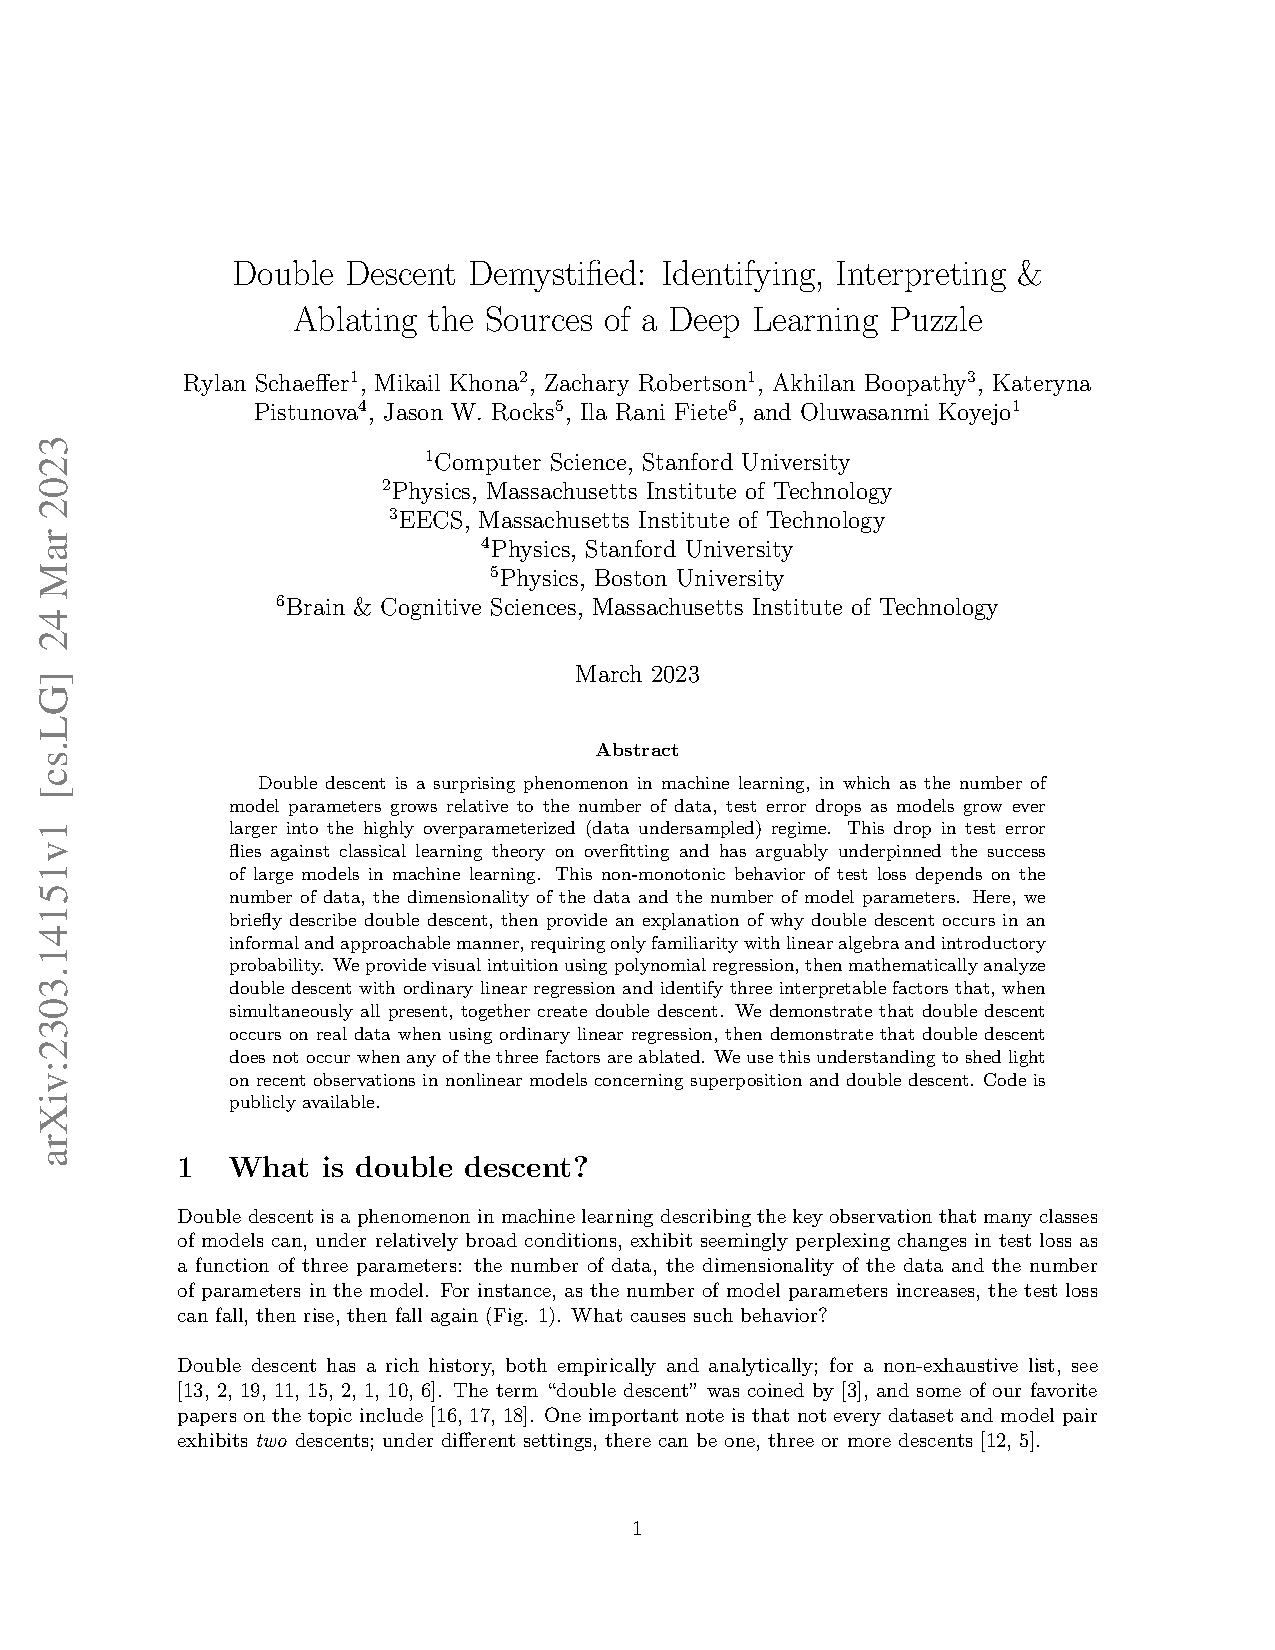
\includegraphics[scale=0.22]{ddd.png}
\end{center}

\end{frame}


\begin{frame}{Double descent in polynomial regression - Empirical}
\begin{center}
\includegraphics[scale=0.22]{polyreg.png}
\end{center}
\end{frame}


\begin{frame}{Terminology}
    \begin{itemize}
        \item Let $P$ be the number of models parameters
        \item Let $N$ be the number of training data
        \item Let $D$ be the dimensionality of the data
    \end{itemize}
    
    \pause
    
    \begin{itemize}
        \item A model is \emph{underparameterized} if $\frac{N}{P} > 1$
        \item A model is \emph{overparameterized} if $\frac{N}{P} < 1$
        \item A model is at the \emph{interpolation threshold} if $\frac{N}{P} = 1$
    \end{itemize}
    
    \pause
    We will next study linear models, which have a fixed value of $P=D+1$. Therefore, double descent occurs in the direction of increasing $N$.

\end{frame}


\begin{frame}{Double descent in linear regression - Mathematical}

The underparametrized regime is the classic least-squares minimization problem:

$$\hat{\vec{\beta}}_{under} = \text{arg} \text{min}_{\vec{\beta}}||X \vec{\beta} - Y||^2_2, $$

which is solved by

$$\vec{\beta}_{under} = (X^T X)^{-1} X^T Y.$$

\pause

For the overparameterized regime, the above optimization problem has infinite solutions. Therefore, we need to choose a different optimization problem:

$$\hat{\vec{\beta}}_{over} = \text{arg} \text{min}_{\vec{\beta}}||\vec{\beta}||^2_2 \text{   s.t.   } \forall n \in (1,\dots,N) \text{   } \vec{x}_n \vec{\beta} = y_n$$

which is solved by

$$\vec{\beta}_{over} = X^T (X X^T)^{-1}Y.$$

\end{frame}


\begin{frame}{Why this choice?}

    $$\hat{\vec{\beta}}_{over} = \text{arg} \text{min}_{\vec{\beta}}||\vec{\beta}||^2_2 \text{   s.t.   } \forall n \in (1,\dots,N) \text{   } \vec{x}_n \vec{\beta} = y_n$$

We choose this optimization problem because \emph{it is the optimization problem that gradient decent implicity minimizes}!
    
\end{frame}


\begin{frame}{Double descent in nonlinear models - Intuition}
TODO
\end{frame}


\begin{frame}{Summary}
TODO
\end{frame}


\begin{frame}{Thank you for listening!}
    \includegraphics[width=\textwidth]{stackmorelayers.jpg}
\end{frame}


\end{document}